% Research Letter -- JACC: Clinical Electrophysiology
% Current live limits (Aug 26, 2026): <=1,000 words including text,
% references, and figure legend; <=5 references; <=10 authors;
% 1 simple figure in no more than 2 parts OR 1 simple table;
% no abstract; no supplemental material.
%
% NOTE: JACC requests Times New Roman 12 pt for submission. This LaTeX draft
% uses a Times-compatible font. Use Times New Roman 12 pt in the final DOCX.

\documentclass[12pt]{article}

\usepackage[T1]{fontenc}
\usepackage[utf8]{inputenc}
\usepackage{newtxtext,newtxmath}
\usepackage[margin=1in]{geometry}
\usepackage{setspace}
\usepackage{graphicx}
\usepackage[super,sort&compress]{natbib}
\usepackage[hidelinks]{hyperref}
\usepackage{caption}
\usepackage{lineno}

\pagestyle{plain}
\setlength{\parindent}{0.5in}
\setlength{\parskip}{0pt}
\renewcommand{\refname}{\normalsize References}
\captionsetup{labelformat=empty,singlelinecheck=false,justification=raggedright,
              font=normalsize}

\begin{document}

% ============================ TITLE PAGE ============================
% Single-spaced, 12 pt, left aligned, one field per line -- JACC asks for
% a single-spaced title page with the rest of the text double-spaced.
\begin{singlespace}
\noindent{\bfseries\large Reader Disagreement Identifies Electrocardiograms
at Increased Risk of Automated Diagnostic Error}

\vspace{2em}

\noindent Khanh Duy Tran, MEng$^{a}$

\vspace{1em}

%\noindent $^{a}$Department, Institution, City, Country \\
% $^{b}$Department, Institution, City, Country

\vspace{2em}

% \noindent\textbf{Running title:} Reader Disagreement and Automated ECG Error

\vspace{0.8em}

% \noindent\textbf{Address for correspondence:} \\
% Name, Degree \\
% Department, Institution \\
% Street, City, Postcode, Country \\
% E-mail: name@institution.edu

\vspace{0.8em}
\end{singlespace}

\newpage
\doublespacing
% Line numbers start with the body; the title page fields are not numbered.
\linenumbers

% ============================ RESEARCH LETTER ============================
Reader disagreement during ECG interpretation may identify cases that are
intrinsically difficult to classify, yet conventional evaluation typically
collapses the adjudication process into a single final reference label.
Automated ECG interpretation has achieved high diagnostic performance and has
also been extended beyond categorical diagnosis to estimation of clinically
relevant values.\cite{ribeiro2020,wei2022} Prior work has shown limited expert
agreement in difficult AI--reader discordant ECGs, while uncertainty estimation
offers a complementary strategy for referring lower-confidence automated
interpretations for expert review.\cite{vranken2021,mayourian2025} We therefore first examined 
whether uncertainty-based referral isolates an
error-prone subset of ECGs and, at full coverage, whether reader disagreement
is enriched among error-containing ECGs and associated with increased
patient-level error risk.

This retrospective secondary analysis used data from the Clinical Outcomes in
Digital Electrocardiology (CODE) study, obtained through the Telehealth Network
of Minas Gerais, a public telehealth system serving primary-care facilities
across Minas Gerais, Brazil. Standard 12-lead ECGs were recorded predominantly
using TEB ECGPC (Tecnologia Eletrônica Brasileira, São Paulo, Brazil) or
ErgoPC 13 (Micromed Biotecnologia, Brasília, Brazil) devices.\cite{ribeiro2020} 
CODE-15\%, comprising 345,779 examinations from 233,770 patients recorded
between 2010 and 2016, served as the model-development cohort.\cite{code15} 
Independent evaluation used CODE-test, comprising 827 ECGs from 827 unique
patients collected in 2018. Each ECG was independently interpreted by
2 cardiologists for first-degree atrioventricular block, right bundle branch
block, left bundle branch block, sinus bradycardia, atrial fibrillation, and
sinus tachycardia, with disagreements adjudicated by a third senior specialist.
\cite{ribeiro2020} The present analysis used only publicly available, de-identified data and
involved no recruitment, intervention, or access to identifiable patient
information; the source CODE study was approved by the Research Ethics
Committee of the Universidade Federal de Minas Gerais
(protocol 49368496317.7.0000.5149).\cite{ribeiro2020}

An ensemble of 5 lightweight 1-dimensional convolutional neural networks with
the same architecture was trained using different random seeds, and their
predicted probabilities were averaged. Following prior work, model confidence
was defined from the diagnosis-specific decision threshold, and whole ECGs were
referred according to their least confident diagnosis.\cite{vranken2021}

Selective analysis was performed at the ECG level. For each ECG, confidence was
defined by its least confident diagnosis, and progressively lower-confidence
ECGs were referred according to the previously described uncertainty
framework.\cite{vranken2021} Selective risk was defined as the proportion of
retained ECGs containing at least 1 incorrect diagnosis among the 6 labels.
Confidence intervals were obtained by bootstrap resampling of whole ECGs so
that all 6 labels from each ECG remained clustered.

To characterize ECGs contributing to the error burden, reader disagreement was
examined at the patient level. A prevalence ratio (PR) quantified enrichment of
reader disagreement among ECGs containing any model error relative to the
overall cohort. A risk ratio (RR) compared the occurrence of any model error
between ECGs with reader disagreement and those with complete reader consensus.
PRs, RRs, and their 95\% confidence intervals were estimated from the same
ECG-level bootstrap.

Uncertainty-based referral concentrated model errors in the lowest-confidence
ECGs. At full coverage, 61 of 827 ECGs (7.4\%) contained at least 1 diagnostic
error; this decreased to 40 ECGs (5.1\%) at 95\% coverage and 29 ECGs (3.9\%)
at 90\% coverage (Figure 1A). The progressive reduction in error burden as
lower-confidence ECGs were referred indicates that model confidence separated
more from less reliable automated interpretations.

Reader disagreement was uncommon overall but enriched among ECGs containing
model error. Disagreement occurred in 33 of 827 ECGs (4.0\%) overall and in
11 of 61 ECGs with any model error (18.0\%; PR: 4.5; 95\% CI: 2.6--6.8).
Conversely, any model error occurred in 11 of 33 ECGs with reader disagreement
(33.3\%) compared with 50 of 794 ECGs with complete reader consensus
(6.3\%; RR: 5.29; 95\% CI: 2.70--8.85) (Figure 1B). Thus, disagreement was
disproportionately represented among error-containing ECGs and identified a
small subgroup with substantially greater patient-level error risk.

In 9 of the 11 ECGs with both reader disagreement and model error, the error
involved the disputed diagnosis; in the remaining 2, the model error involved
a different diagnosis. This pattern suggests that disagreement usually marks
difficulty in the same diagnostic decision, while occasionally identifying a
more generally difficult ECG. Importantly, disagreement should not be
interpreted as evidence that the adjudicated reference was incorrect. Rather,
it marks an interpretive boundary at which independent cardiologists did not
initially converge, consistent with prior expert readjudication studies showing
limited agreement in difficult AI--reader discordant ECGs.\cite{mayourian2025}

Model uncertainty and reader disagreement therefore captured complementary
aspects of automated ECG reliability. Uncertainty provided an operational
mechanism for referring lower-confidence ECGs, whereas reader disagreement was
both enriched among error-containing ECGs (PR: 4.5) and associated with greater
patient-level error risk (RR: 5.29). The small number of disagreement cases
(33 patients, including 11 with any model error) limits precision and precludes
diagnosis-specific inference; these findings should therefore be considered
hypothesis-generating and require external validation in datasets preserving
independent reader annotations. Nonetheless, combining uncertainty-based
referral with reader-level disagreement may provide a more clinically
informative assessment of automated ECG reliability than treating all
adjudicated labels as equally certain.
% ============================ REFERENCES ============================
% Order here sets the numbering: entries must be in order of first citation.
\begin{singlespace}
\begin{thebibliography}{4}

\bibitem{ribeiro2020}
Ribeiro AH, Ribeiro MH, Paix\~ao GMM, et al. Automatic diagnosis of the 12-lead ECG using a deep neural network. \textit{Nat Commun}. 2020;11:1760.

\bibitem{wei2022}
Wei G, Di X, Zhang W, et al. Estimating critical values from electrocardiogram using a deep ordinal convolutional neural network. \textit{BMC Med Inform Decis Mak}. 2022;22:295.

\bibitem{vranken2021}
Vranken JF, van de Leur RR, Gupta DK, et al. Uncertainty estimation for deep learning-based automated analysis of 12-lead electrocardiograms. \textit{Eur Heart J Digit Health}. 2021;2:401-415.

\bibitem{mayourian2025}
Mayourian J, La Cava WG, de Ferranti SD, et al. Expert-level automated diagnosis of the pediatric ECG using a deep neural network. \textit{JACC Clin Electrophysiol}. 2025;11:1308-1320.

\bibitem{code15}
Ribeiro AH, Paix\~ao GMM, Lima EM, et al. CODE-15\%: a large scale annotated dataset of 12-lead ECGs. Zenodo. 2021.

\end{thebibliography}
\end{singlespace}

% ============================ FIGURE LEGEND ============================


% The journal requires the figure as a separate upload. The image below is
% included only to make this drafting PDF self-contained for review.
% Not a float: placed at the top of its own page rather than drifting to the
% vertical centre. Drawn at 7.4 in and centred across the margins, because
% \textwidth here is 6.5 in and scaling to that would put the lettering back
% below the journal's 10 pt floor.
\clearpage
\nolinenumbers        % a stray line number was printing beside the figure
\thispagestyle{plain}
\noindent\makebox[\textwidth][c]{%
  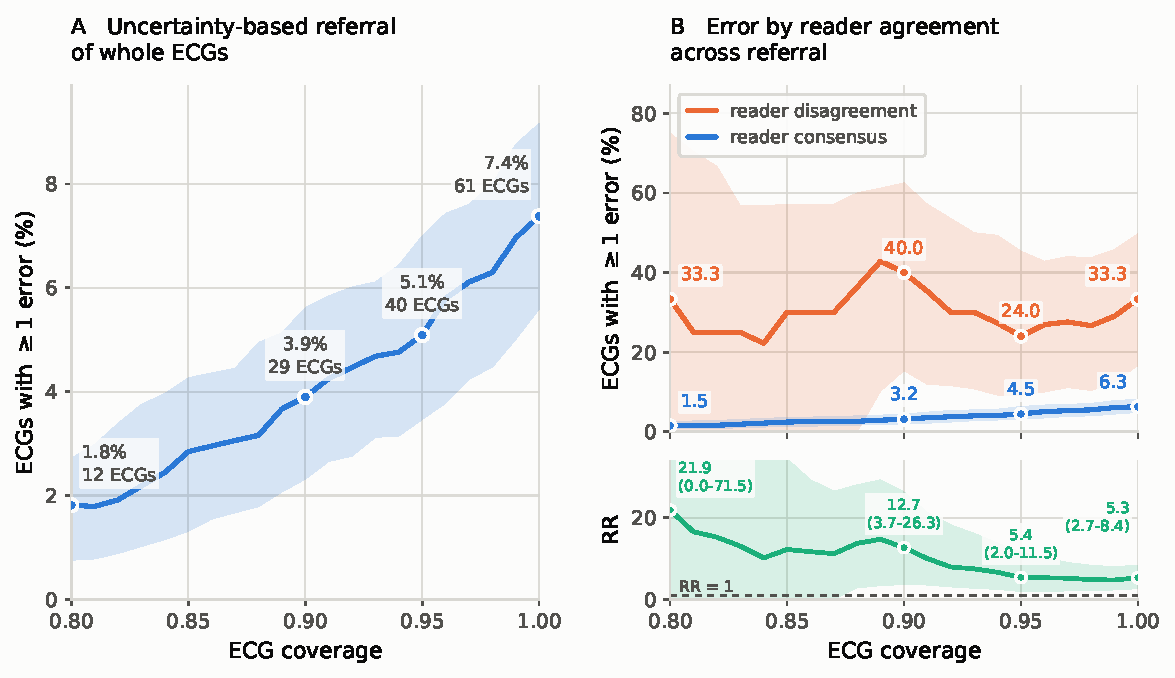
\includegraphics[width=7.4in]{figures/figure1.pdf}}
\noindent\textbf{Figure 1. Uncertainty-Based Referral and Reader Disagreement in Automated ECG Diagnosis.}
\textbf{(A)} Proportion of retained ECGs containing at least 1 automated
diagnostic error as lower-confidence ECGs are progressively referred; referral
is by whole ECG, ranked on its least confident diagnosis, and the upper axis
shows the corresponding proportion referred. Annotated points give the value
and the number of affected ECGs at full, 95\%, and 90\% coverage. Shading represents 95\% ECG-level
bootstrap confidence intervals. \textbf{(B)} Patient-level association between
reader disagreement and automated diagnostic error. Left, prevalence of reader
disagreement among all ECGs and among ECGs containing at least 1 model error.
Right, prevalence of any model error among ECGs with complete reader consensus
and those with any disputed diagnosis. Error bars represent 95\% confidence
intervals. PR = prevalence ratio; RR = risk ratio.
\vfill



\end{document}
